\section{Implementation}

\begin{frame}[b]{Central Data Structure: Adaptive}
  \vfill
  \begin{itemize}
    \item Central Data Structure: Adaptive neighbor-linked quadtree
    \item Data stored in nodes
    \begin{itemize}
      \item Children (only in inner nodes)
      \item Neighbors
      \item Expansions (coefficients $\hat{\vct q}$ and $\hat{\vct u}$)
      \item Particles (only in leaf nodes)
    \end{itemize}
  \end{itemize}

  \vfill
  \begin{figure}
    \centering
    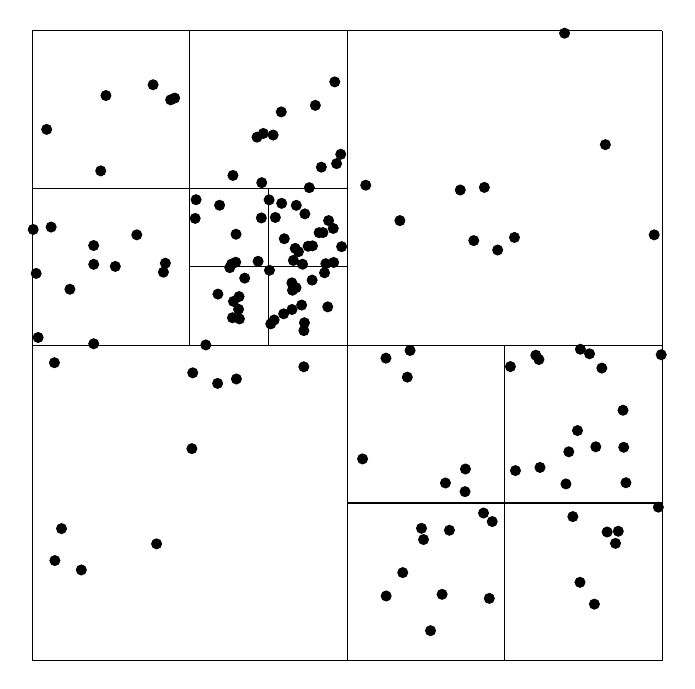
\begin{tikzpicture}
      \draw[step=4] (0,0) grid (8,8);
      \foreach \x in {1,...,10} {
        \fill (rnd*4, rnd*4) circle (2pt);
      }
      \foreach \x in {1,...,10} {
        \fill (4+rnd*4, 4+rnd*4) circle (2pt);
      }

      \draw[step=2] (0,4) grid (4,8);
      \draw[step=2] (4,0) grid (8,4);
      \foreach \x in {1,...,40} {
        \fill (rnd*4, 4+rnd*4) circle (2pt);
      }
      \foreach \x in {1,...,40} {
        \fill (4+rnd*4, rnd*4) circle (2pt);
      }

      \draw[step=1] (2,4) grid (4,6);
      \foreach \x in {1,...,40} {
        \fill (2+rnd*2, 4+rnd*2) circle (2pt);
      }
    \end{tikzpicture}
  \end{figure}
\end{frame}

\begin{frame}[fragile]{Pseudocode}
  \begin{lstlisting}[caption = Fast Multipole Method]
repairTree();

upwardPass();
downwardPass();
  \end{lstlisting}

  \begin{lstlisting}[caption = Upward Pass]
tree.traversePostOrder(Tree t ->
  t.outgoingExpansion.reset();

  if (t is leaf)
    for p in t.particles
      t.outgoingExpansion.add(p);
  else
    for child in t.childs
      t.outgoingExpansion.add(expOut);
);
  \end{lstlisting}
\end{frame}

\begin{frame}[fragile]{Pseudocode}
  \begin{lstlisting}[caption = Downward Pass]
tree.incomingExpansion.reset();
tree.traversePreOrder(Tree t ->
  if (t is inner node)
    for child in t.childs
      child.incomingExpansion.reset();
      child.incomingExpansion.add(t.incomingExpansion);

      for parentNeigh in t.neighs
        for neighChild in parentNeigh.childs
          if (neighChild not in child.neighs)
            child.incomingExpansion.add(neighChild.expOut);
  else
    for p in t.particles
      t.incomingExpansion.applyForce(p);
      calculateDirectForces(t, p);
);
  \end{lstlisting}
\end{frame}

\begin{frame}[fragile]{Pseudocode}
  \begin{lstlisting}[caption = Calculation of Direct Forces]
calculateDirectForces(t, p):
// same cell
for q in t.particles following p
  calculateForce(p, q);

// neighbors
for neigh in t.neighs
  if (index(neigh) < 4 or neigh is inner node)
    neigh.traversePreOrder(Tree node ->
      for q in node.particles
        calculateForce(p, q);
    );
  \end{lstlisting}
\end{frame}

\begin{frame}{TODO}
  Adaptive neighbor-linked Quadtree \\
  Successive rebuilds \\
  $\mathcal O(n)$
\end{frame}

\section{Results}

\begin{frame}{TODO}
  Initial conditions \\
  Video \\
  Parameters (particles per leaf, order of expansions) \\
  Scaling graph \\
  Comparison to direct computation and cell list
\end{frame}

\begin{frame}

  \begin{figure}[H]
    \centering
    \begin{tikzpicture}[scale=0.7]
      \begin{axis}[ xlabel = {$\# Particles$}
                  , ylabel = {Wall time [\si{s}]}
                  , xmode  = log
                  , ymode  = log
                  , width  = 0.7\textwidth
                  , height = 0.7\textwidth
                  , ymin   = 0
                  , minor y tick num = 4
                  , grid   = both
                  , grid style = {line width=.2pt, draw=gray!10}
                  , major grid style = {line width=.2pt,draw=gray!50}
                  , legend pos = {north west}
                  , legend cell align = {left}
                  , every axis plot/.append style={ultra thick}
                  ]
        \addplot table [x=nParticles,y=time] {data/scaling_time-per-particles-leaf001-dt0.1-nSteps500.txt};
        \addplot table [x=nParticles,y=time] {data/scaling_time-per-particles-leaf005-dt0.1-nSteps500.txt};
        \addplot table [x=nParticles,y=time] {data/scaling_time-per-particles-leaf010-dt0.1-nSteps500.txt};
        \addplot table [x=nParticles,y=time] {data/scaling_time-per-particles-leaf017-dt0.1-nSteps500.txt};
        \addplot table [x=nParticles,y=time] {data/scaling_time-per-particles-leaf025-dt0.1-nSteps500.txt};
        \addplot table [x=nParticles,y=time] {data/scaling_time-per-particles-leaf050-dt0.1-nSteps500.txt};
        \addplot table [x=nParticles,y=time] {data/scaling_time-per-particles-leaf064-dt0.1-nSteps500.txt};
        \addplot table [x=nParticles,y=time] {data/scaling_time-per-particles-leaf100-dt0.1-nSteps500.txt};
        \addlegendentry{\SI{001}{maxLeafsPerNode}};
        \addlegendentry{\SI{005}{maxLeafsPerNode}};
        \addlegendentry{\SI{010}{maxLeafsPerNode}};
        \addlegendentry{\SI{017}{maxLeafsPerNode}};
        \addlegendentry{\SI{025}{maxLeafsPerNode}};
        \addlegendentry{\SI{050}{maxLeafsPerNode}};
        \addlegendentry{\SI{064}{maxLeafsPerNode}};
        \addlegendentry{\SI{100}{maxLeafsPerNode}};

        \addplot+[domain=3e1:1e6] {ln(x)*x   * 1e-3};
        \addlegendentry{Comparison Line Nlog(N)};

        \addplot[domain=3e1:5e2] {x^2 * 2e-6};
        \addplot[domain=5e2:1e6] {x   * 1e-3};
        \fill (500, 0.5) circle (2pt);
        \addlegendentry{Comparison Line};

      \end{axis}
    \end{tikzpicture}
    \caption{Comparison Line, part left of the circle has a quadratic slope while the part right of the circle has a linear slope.}%
    \label{fig:gs_plain}
  \end{figure}\todo{describe the plot and maybe talk about the unregularity at $2^{14}$.}

  \todo{add speedup plot cell vs. fmm, as well}
\end{frame}






